\section{Additional spatial and dynamical results}
\label{sec:additional}

\noindent\begin{minipage}{\textwidth}

\begin{appendixfigure}
\centering
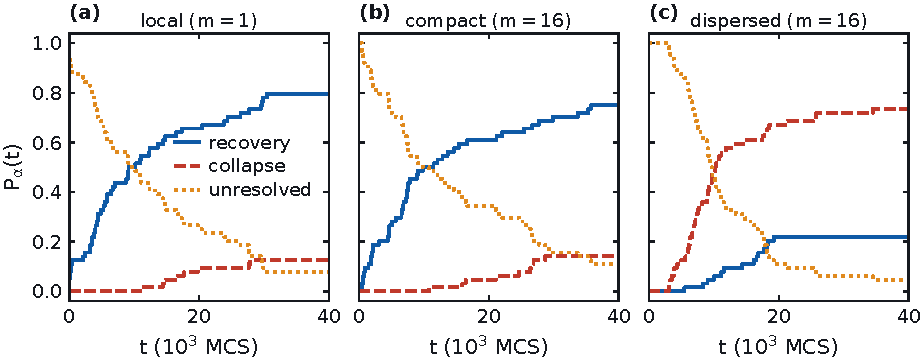
\includegraphics[width=0.85\textwidth]{fig03_fate_kinetics.pdf}
\caption{Outcome kinetics following (a) a single-site, (b) a compact 16-site, and (c) a dispersed 16-site perturbation. Each panel uses 64 independent realizations at the reference parameters. Recovery, collapse, and unresolved probabilities partition the full ensemble. Steps occur at recorded event times; the first event label is retained.}
\label{fig:kinetics}
\end{appendixfigure}



\begin{appendixfigure}
\centering
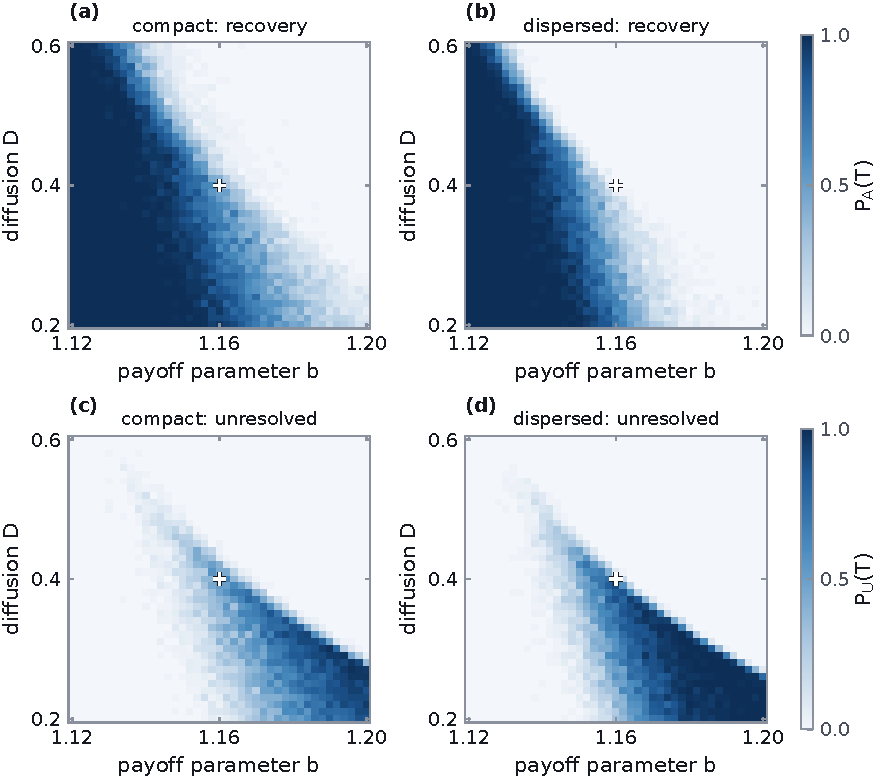
\includegraphics[width=0.8\textwidth]{figS01_recovery_unresolved.pdf}
\caption{Recovery (a,b) and unresolved (c,d) probabilities for compact and dispersed perturbations. Together with Fig.~\ref{main-fig:phase}, every parameter cell satisfies $P_A+P_B+P_U=1$ at $T=10000$ MCS. Crosses mark the reference parameters. Each cell contains 64 realizations per geometry; no interpolation is applied.}
\label{fig:outcomes}
\end{appendixfigure}

\end{minipage}

\clearpage
\noindent\begin{minipage}{\textwidth}

\begin{appendixfigure}
\centering
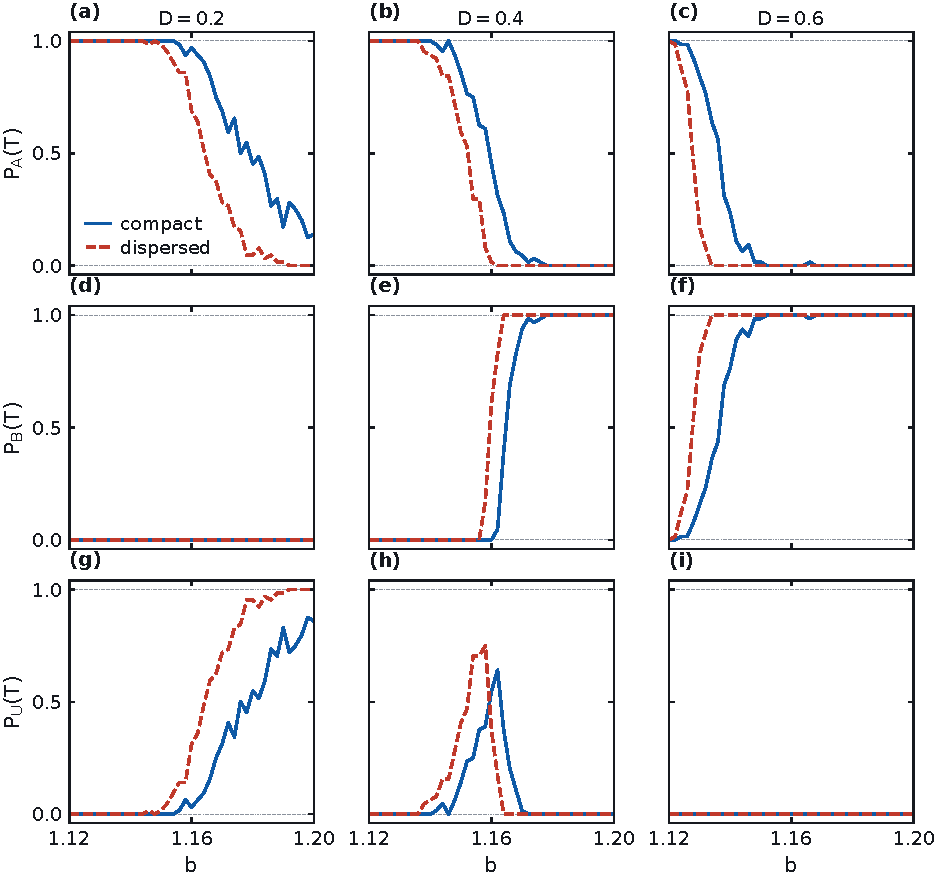
\includegraphics[width=0.8\textwidth]{fig05_phase_sections.pdf}
\caption{Competing outcomes along three diffusion sections. Columns show $D=0.2,0.4,0.6$; rows show recovery, collapse, and unresolved probabilities. Each panel compares the two geometries at all 41 measured payoff values, with 64 realizations per value and $T=10000$ MCS. Lines connect the sampled values. These sections distinguish transfer into unresolved evolution from transfer into collapse.}
\label{fig:sections}
\end{appendixfigure}



\begin{appendixfigure}
\centering
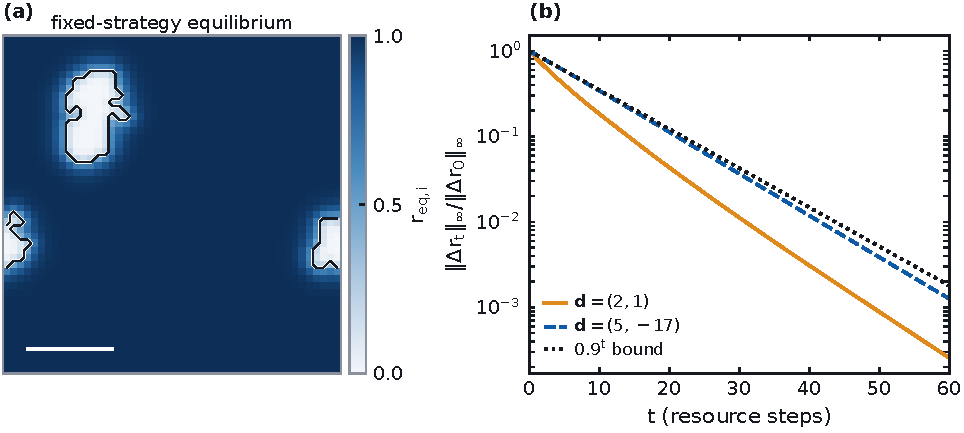
\includegraphics[width=0.8\textwidth]{figS06_resource_controls.pdf}
\caption{Resource adaptation at fixed strategies. (a) Equilibrium field for the strategy configuration in Fig.~\ref{main-fig:alignment}; scale bar: 12 sites. (b) Median normalized maximum-norm difference between translated and original fields over 48 configurations. The dotted curve is the contraction bound $0.9^t$. The strategy pattern is fixed throughout; this is not a relaxation-time measurement for the coupled system.}
\label{fig:resourcecontrols}
\end{appendixfigure}

\end{minipage}

\clearpage

\begin{appendixfigure}
\centering
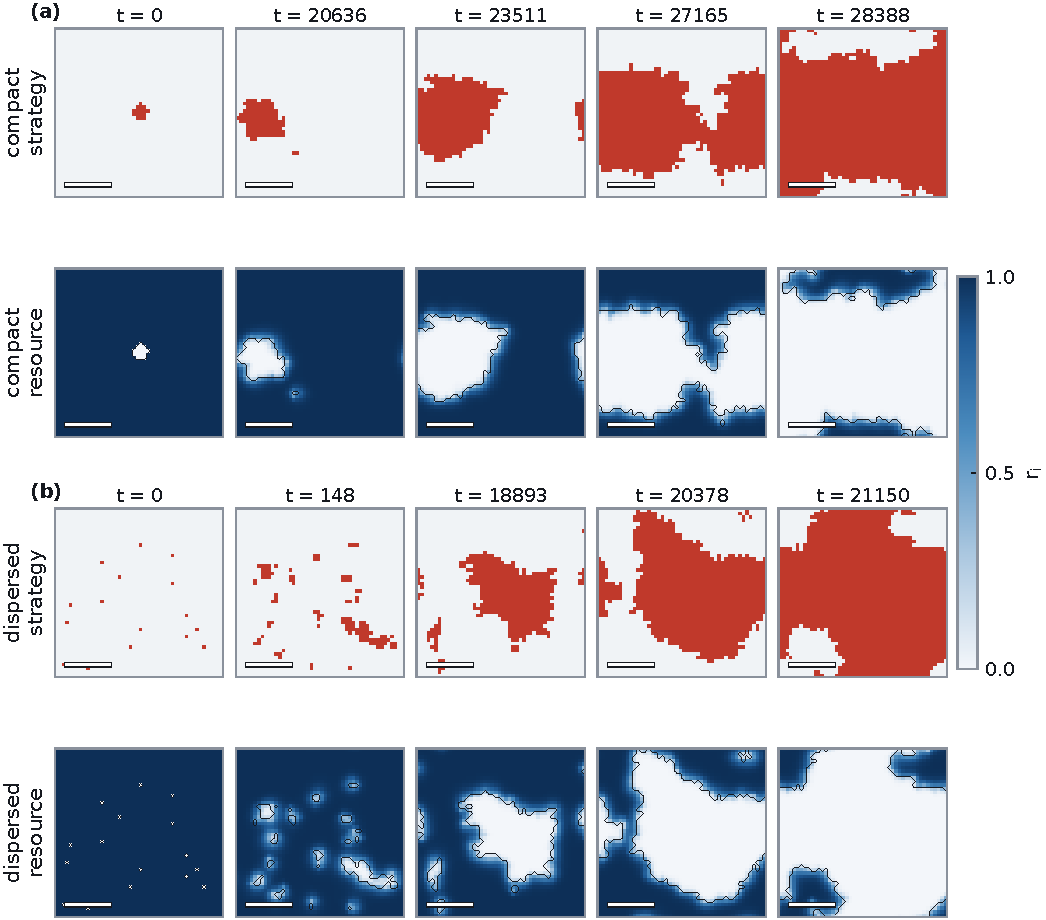
\includegraphics[width=0.87\textwidth]{figS03_full_growth_fields.pdf}
\caption{Strategy and resource evolution for the examples in Fig.~\ref{main-fig:fields}: (a) compact and (b) dispersed preparation. Columns show the initial state and first 5\%, 20\%, 50\%, and 80\% defector crossings. Red sites are defectors; resource maps share $0\le r_i\le1$. Time is in MCS and scale bars span 12 sites. Each trajectory uses one fixed spatial translation.}
\label{fig:fullfields}
\end{appendixfigure}


\clearpage
\noindent\begin{minipage}{\textwidth}

\begin{appendixfigure}
\centering
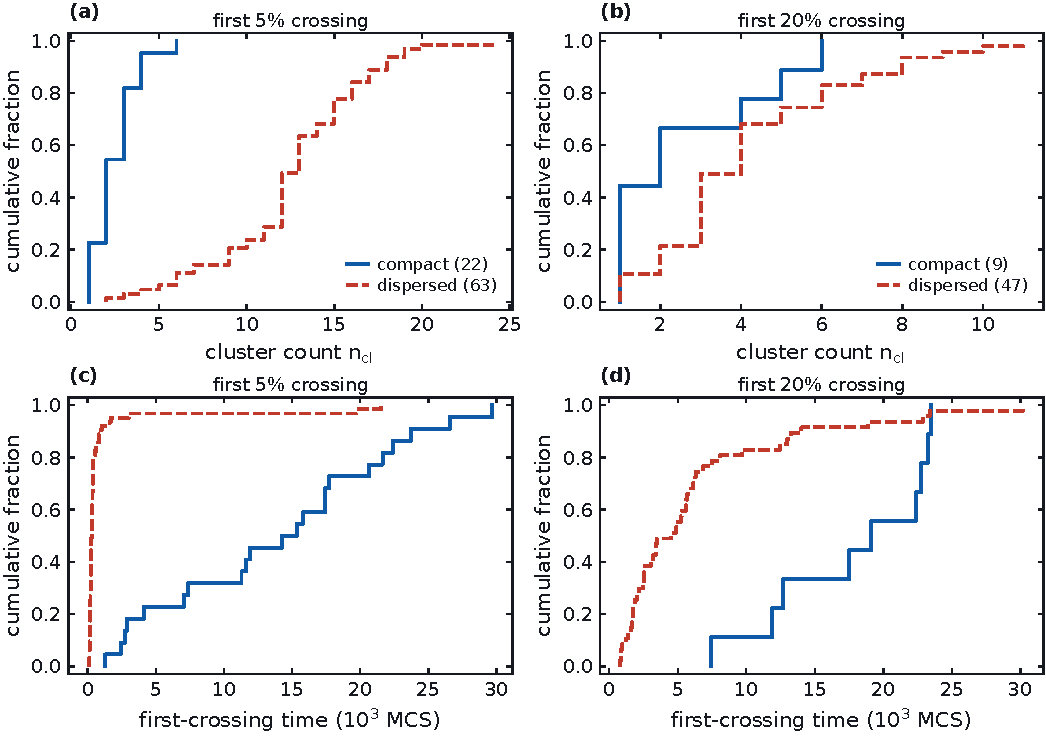
\includegraphics[width=0.8\textwidth]{figS04_growth_distributions.pdf}
\caption{Conditional spatial and first-passage distributions. (a,b) Periodic cluster counts at first 5\% and 20\% crossings. (c,d) Corresponding arrival times. Curves include every trajectory reaching the specified threshold by $T=40000$ MCS; legend counts give the denominators. The reaching subsets differ between geometries and thresholds.}
\label{fig:growthdistributions}
\end{appendixfigure}



\begin{appendixfigure}
\centering
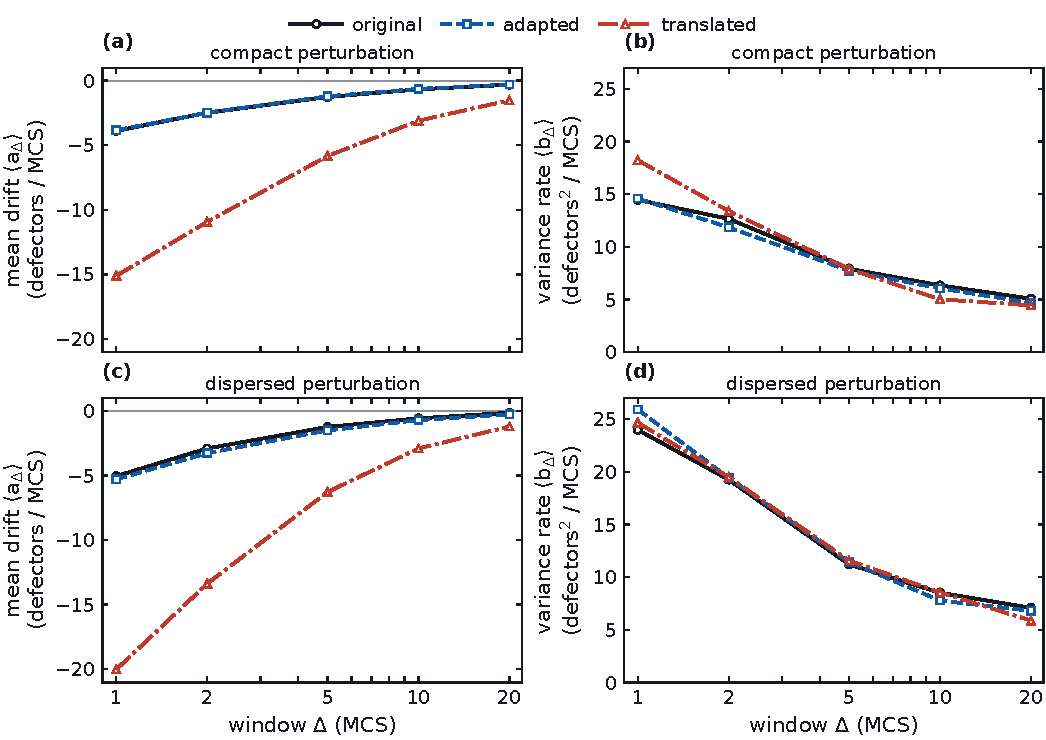
\includegraphics[width=0.8\textwidth]{fig06_conditional_moments.pdf}
\caption{Finite-window drift (left) and conditional variance rate (right) after resource redistribution. Rows distinguish compact and dispersed origins. Each mean uses 15 configurations at the first 5\% crossing and 64 continuations per configuration and treatment. Circles, squares, and triangles denote original, fixed-strategy-adapted, and translated $(17,12)$ fields. Lines join the five measured windows; these rates differ from the first-visit moments.}
\label{fig:windows}
\end{appendixfigure}

\end{minipage}

\clearpage

\begin{appendixfigure}
\centering
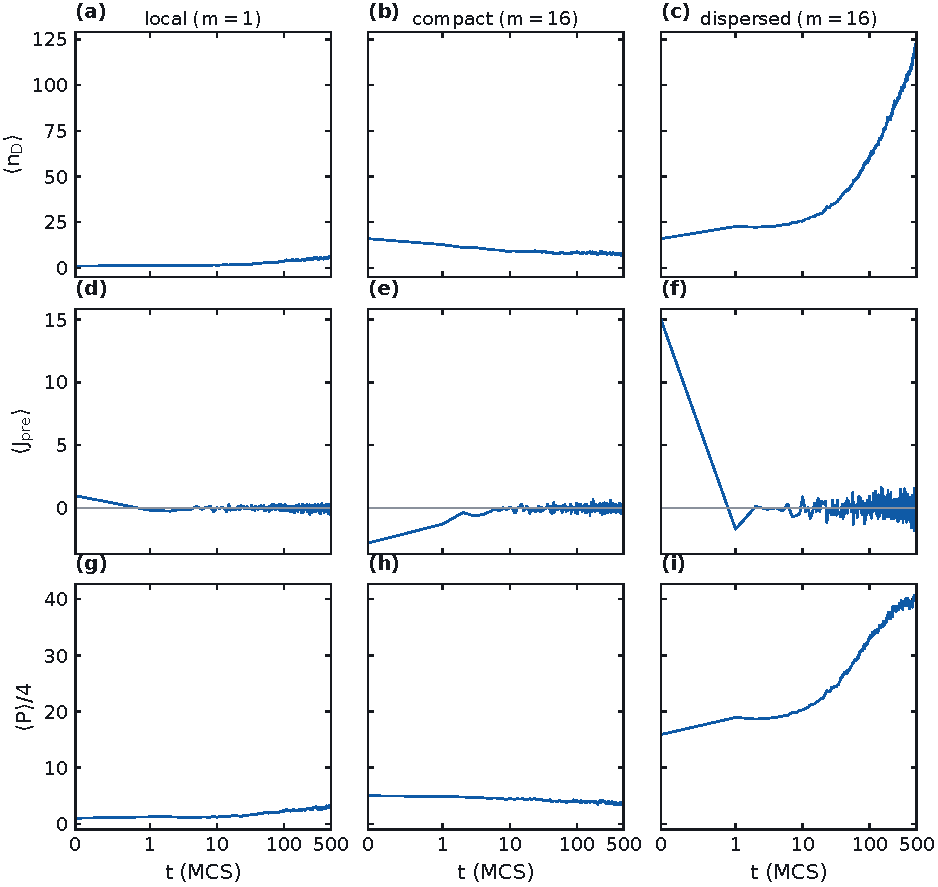
\includegraphics[width=0.86\textwidth]{fig04_interface_dynamics.pdf}
\caption{Early population growth, interface bias, and activity. Columns show single-site, compact, and dispersed preparations; rows show mean $n_D$, $J_{\rm pre}$, and $P/4$. Every recorded MCS through $t=500$ is included for all 64 realizations, including absorbed paths. Time is linear up to one MCS and logarithmic thereafter. The quantity $P/4=N\mathbb E[Z^2]$ measures frozen first-visit activity, not a complete-cycle variance.}
\label{fig:interface}
\end{appendixfigure}


\clearpage
\noindent\begin{minipage}{\textwidth}

\begin{appendixfigure}
\centering
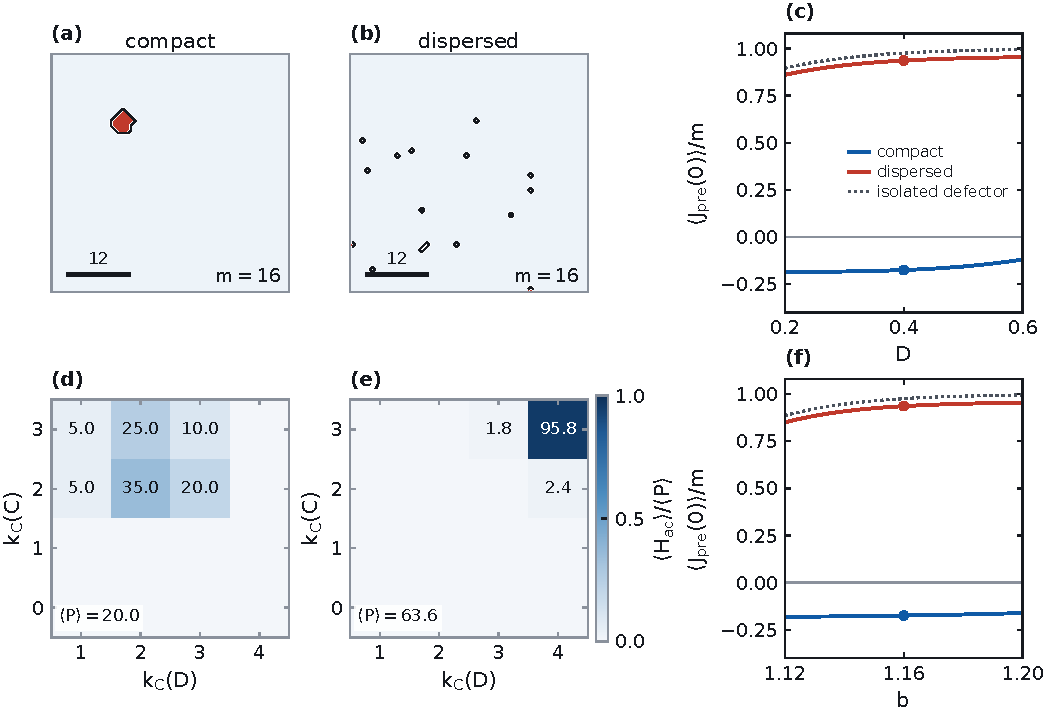
\includegraphics[width=0.84\textwidth]{fig09_initial_interfaces.pdf}
\caption{Initial interface geometry and growth bias. (a,b) Compact and dispersed 16-site preparations on the $48\times48$ lattice; red sites are defectors, pale-blue sites are cooperators, and bars span 12 sites. (c,f) Exact motif-based bias per initial defector as a function of $D$ at $b=1.16$ and of $b$ at $D=0.4$; dots mark the reference parameters and dotted curves show an isolated defector. These are frozen-initial-state diagnostics. (d,e) Fractions of interfacial edges with $a=k_C(C)$ and $c=k_C(D)$ cooperative neighbors. Numbers give percentages; the color scale is a fraction. Motifs and biases use all 64 preparations per geometry.}
\label{fig:initialinterfaces}
\end{appendixfigure}



\begin{appendixfigure}
\centering
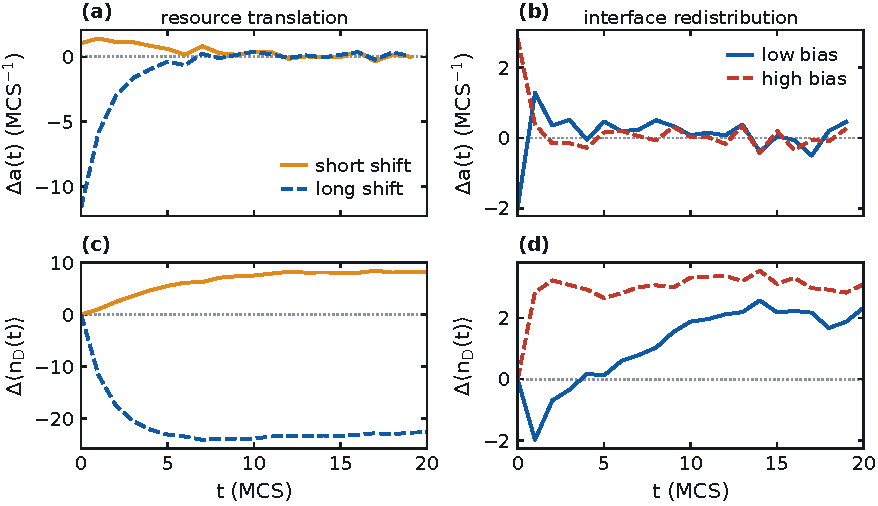
\includegraphics[width=0.8\textwidth]{fig07_cumulative_response.pdf}
\caption{Population response to translation (left) and boundary redistribution (right), relative to the original field. (a,b) Change in mean increment per MCS, $\Delta a(t)$. (c,d) Accumulated difference $\mathcal I_a(t)$. Means use 48 configurations and 16 continuations per treatment; translations average four rotations of $(2,1)$ (short) or $(5,-17)$ (long). Every recorded time through 20 MCS is shown.}
\label{fig:response}
\end{appendixfigure}

\end{minipage}

\clearpage

\begin{appendixfigure}
\centering
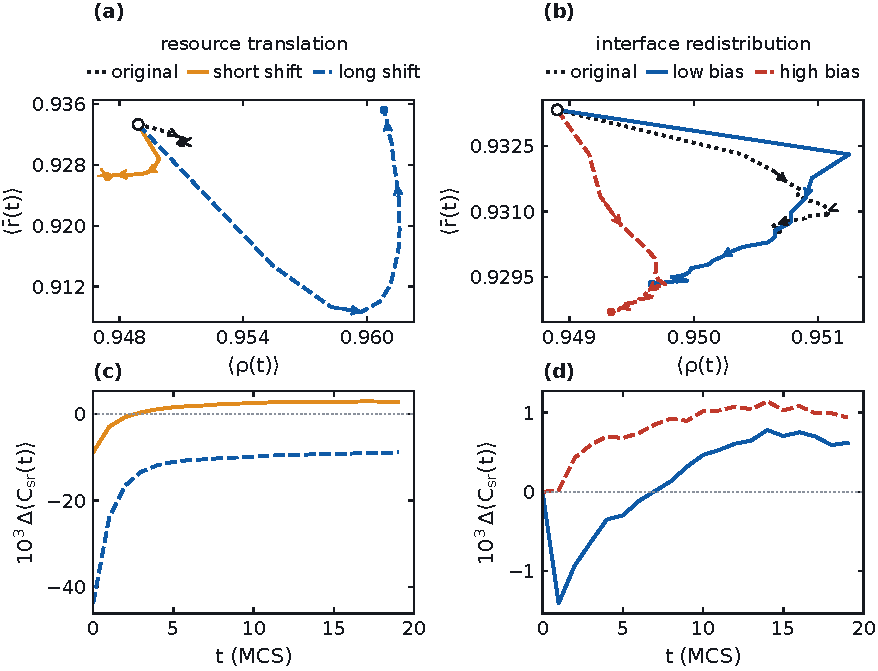
\includegraphics[width=0.8\textwidth]{fig08_coupled_response.pdf}
\caption{Coupled response of the ensembles in Fig.~\ref{fig:response}: translation (left), boundary redistribution (right). (a,b) Mean cooperation--resource paths over 20 MCS. Circles mark the common initial state (open) and endpoints (filled); arrows indicate increasing time. (c,d) Strategy--resource covariance changes, reconstructed per trajectory. These mean paths do not define a closed flow.}
\label{fig:feedback}
\end{appendixfigure}

\par
